\documentclass[12pt]{article}
%\documentclass[border=0.1cm]{standalone}
\usepackage{wasysym}
\usepackage{phonenumbers}
\usepackage{marvosym}
\usepackage{xcolor}
\usepackage[super]{nth}
\usepackage[paperwidth=8.5in,paperheight=11in,margin=0.45in]{geometry} 
\usepackage[USenglish]{babel}
\usepackage[USenglish]{isodate}% http://ctan.org/pkg/isodate
\usepackage[final]{pdfpages}
\usepackage{hyperref}
\hypersetup{
  colorlinks   = true, %Colours links instead of ugly boxes
  urlcolor     = black, %Colour for external hyperlinks
  linkcolor    = black, %Colour of internal links
  citecolor    = black %Colour of citations
}
\usepackage[activate={true,nocompatibility},final,tracking=true,kerning=true,spacing=true,factor=1100,stretch=10,shrink=10]{microtype}
\frenchspacing
\usepackage[nodayofweek,level]{datetime}
\usepackage{calc,url}
\newcounter{qz}\setcounter{qz}{0}
\newcommand{\qz}{%\
\setcounter{qz}{\value{qz}+1}
\textbf{In-class  \theqz} \,}

\newcounter{hw}\setcounter{hw}{0}
\newcommand{\hw}{%\
\setcounter{hw}{\value{hw}+1}
\textbf{IC \thehw}}

\newcounter{on}\setcounter{on}{0}
\newcommand{\on}{%\
\setcounter{on}{\value{on}+1}
\textbf{OL \theon}}


\newcounter{ex}\setcounter{ex}{0}
\newcommand{\ex}{%\
\setcounter{ex}{\value{ex}+1}
Exam \theex}

\usepackage[T1]{fontenc} 
\usepackage{fourier}
%\usepackage{tgschola} %to look retro
\newenvironment{mypar}[2]
  {\begin{list}{}%
    {\setlength\leftmargin{#1}
    \setlength\rightmargin{#2}}
    \item[]}
  {\end{list}}


\newcounter{wk}\setcounter{wk}{0}
\newcommand{\wk}{%\
\setcounter{wk}{\value{wk}+1}
\thewk \,\,}

\usepackage[nomessages]{fp}% http://ctan.org/pkg/fp


\usepackage{enumerate}
\usepackage{graphicx}

\usepackage{paralist}
\renewenvironment{description}[0]{\begin{compactdesc}}{\end{compactdesc}}

\newenvironment{alphalist}{
  \begin{enumerate}[(a)]
    \addtolength{\itemsep}{-0.75\itemsep}}
  {\end{enumerate}}
  \cleanlookdateon% Remove ordinal day reference
  \newcommand{\RomanNumeralCaps}[1]
      {\MakeUppercase{\romannumeral #1}}

\usepackage{xspace}
\makeatletter
\DeclareRobustCommand{\maybefakesc}[1]{%
  \ifnum\pdfstrcmp{\f@series}{\bfdefault}=\z@
    {\fontsize{\dimexpr0.8\dimexpr\f@size pt\relax}{0}\selectfont\uppercase{#1}}%
  \else
    \textsc{#1}%
  \fi
}
\newcommand\AM{\maybefakesc{am}\xspace}
\newcommand\PM{\maybefakesc{pm}\xspace}
\makeatother

 \newcommand{\coursename}{College Algebra}
\newcommand{\coursenumber}{MATH 102}
\newcommand{\sectionnumber}{01}
\newcommand{\term}{Spring }
\newcommand{\room}{TBA}
\newcommand{\meetingtime}{This class meets Monday, Wednesday, and Friday in \room \/  from 9:05 \AM to 9:55 \AM.}
\newcommand{\officehours}{Monday, Wednesday, and Friday 10:00\AM-11:00\AM,
    Tuesday and Thursday 12:00 noon-2:00\PM, and by appointment.}

\begin{document}
\cleanlookdateon% Remove ordinal day reference
\shortdate
\printyearoff
\large
\begin{center}
    \textbf{\coursename}  \\
    {\coursenumber--\sectionnumber} \\
     {\term \the\year} \\
\end{center}

\vskip0.25in
\normalsize


\begin{center}
\begin{description}
    \item[Instructor:] Barton Willis, PhD, Professor of Mathematics
    \item[Office:]  Discovery Hall, Room 368
    \item[\phone:]   \phonenumber[country=US]{3088658868}
    \item[\Email:]    \href{mailto:willisb@unk.edu}{willisb@unk.edu}
    \item[Zoom for classes:] For Zoom class meetings, use the Meeting ID: 616 568 5706. 
    \item[Office Hours:] \officehours
  \end{description}
\end{center}

\subsubsection*{Class meeting time and place}

\meetingtime



\subsubsection*{Course Resources}

\noindent Our textbook is \emph{College Algebra}, \nth{11} edition, by Michael 
Sullivan with access to MyLab Math; ISBN: 9780136483151


\subsubsection*{Important Dates}

\begin{mypar}{0.25in}{0.25in} 

    \textbf{First Homework due} \dotfill  \textbf{\printdate{27/1/\the\year}}  \\
    \textbf{Exam 1} \dotfill \textbf{\printdate{17/2/\the\year}}  \\
    \textbf{Exam 2} \dotfill  \textbf{\printdate{24/3/\the\year}} \\
    \textbf{Exam 3} \dotfill \textbf{\printdate{21/4/\the\year}} \\
    \textbf{Final exam} \dotfill  \textbf{\printdate{17/5/\the\year}, 8:00 \AM--10:00 \AM}
\end{mypar}



\subsubsection*{Grading}

Your course grade will be based on online homework, in class work,
three midterm exams, and a comprehensive final exam; specifically:
\begin{mypar}{0.25in}{0.25in}
    \textbf{In class work}  \emph{14 ten point assignments}  \dotfill 140 (total) \\
    \textbf{Online homework} \emph{31 five point assignments}\dotfill 155 (total) \\
    \textbf{Mid-term exams 1,2, and 3} \emph{100 points each} \dotfill 300 (total)\\
    \textbf{Comprehensive Final exam} \dotfill 150 (total)
\end{mypar}
If it is necessary to adjust the number of  homework assignments,  your homework point 
total will be scaled to a total of 165.  For example, if we have only ten homework sets, 
your homework score will be scaled by a factor of \(165/150\). The same holds
for class participation.

\FPeval{\points}{round(165+60+300+150,0)}

\FPeval{\F}{round(\points*0.6-1,0)}
\FPeval{\Dm}{round(\points*0.6,0)}
\FPeval{\D}{round(\points*0.63,0)}
\FPeval{\Dp}{round(\points*0.66,0)}

\FPeval{\Cm}{round(\points*0.7,0)}
\FPeval{\C}{round(\points*0.73,0)}
\FPeval{\Cp}{round(\points*0.76,0)}

\FPeval{\Bm}{round(\points*0.8,0)}
\FPeval{\B}{round(\points*0.83,0)}
\FPeval{\Bp}{round(\points*0.86,0)}

\FPeval{\Am}{round(\points*0.9,0)}
\FPeval{\A}{round(\points*0.93,0)}
\FPeval{\Ap}{round(\points*0.98,0)}
The following table shows the \emph{minimum} number of points (out of \points) that
are required for each of the twelve letter grades D- through A+. For
example, a point total of \Bp\/  points will earn you a grade of B+,  and 
a point total of \Am\/ points will earn you a grade of A-. A point
total of \F\/  or less earns you a failing course grade.
 
 \vspace{0.1in}
     \begin{minipage}{5.5in}
  \centering 
\begin{mypar}{0.25in}{0.25in}
    \begin{minipage}{2.5in}
        D-  \dotfill \Dm \\
        D \dotfill \D \\
        D+ \dotfill \Dp \\
        C- \dotfill \Cm  \\
        C \dotfill \C \\
        C+ \dotfill \Cp 
        \end{minipage}
    \phantom{xxx}
    \begin{minipage}{2.5in}
        B- \dotfill \Bm \\
        B \dotfill  \B \\
        B+ \dotfill  \Bp\\
        A- \dotfill  \Am \\
        A \dotfill  \A \\
        A+ \dotfill  \Ap
    \end{minipage}
\end{mypar} 
\end{minipage}

\subsubsection*{In class work}

Each week, for a portion of class time we will do in class work. Either 
in a small group or individually, you will complete a worksheet in class.
Generally, it will be due at the end of the class period.

Most weeks, we'll do in class work on Wednesday. 

\subsubsection*{Prerequisite}

The prerequisite for this class is either an earned passing grade (D- or higher) in 
MATH 101 or Math ACT score of 20 or greater.  

\subsubsection*{Catalog description}


\textbf{College Algebra (3 credit hours)} A college level algebra course 
which includes a study of linear equations and inequalities, relations and 
functions, graphing of linear and quadratic functions, polynomial and
rational functions, logarithmic and exponential functions, systems of 
equations, matrices, sequences and series, and other selected topics 
all of which are necessary for the study of calculus.

\subsubsection*{LOPER 4 Learning Outcomes}

College Algebra is a LOPER 4 General Studies class. The Learning Outcomes for
all  LOPER 4 classes are
\begin{alphalist}
\item Can describe problems using mathematical, statistical, or programming language.
\item Can solve problems using mathematical, statistical, or programming techniques.
\item Can construct logical arguments using mathematical, statistical, or programming concepts.
\item Can interpret and express numerical data or graphical information using 
   mathematical, statistical, or programming concepts and methods.
\end{alphalist}


\subsubsection{College Algebra specific learning outcomes} 

In this course students will learn the concepts of relations and 
functions, properties and graphing of various types functions, and other topics such 
as systems of equations, matrices, and/or sequences and series. Students will 
investigate applied problems from various disciplines and 
algebraic principles used in the study of calculus, linear programming, and other 
areas of mathematics. Through this course, students will be able to

\begin{alphalist}

\item Solve algebraic equations and inequalities in one or two variables and illustrate these solutions graphically on the real number line and/or the rectangular coordinate system. 

\item Use the Pythagorean Theorem to develop distance computations and circular relationships in two variables on the coordinate system. 

\item   Understand the concepts of slope and the linear relationship, using graphic, algebraic, and verbal descriptions of this relationship. 

\item Apply the definition of the function, function notation, and the connections between graphic, algebraic, and verbal descriptions of functions. 

\item  Understand the domain and the range of a function, how to determine domain using equations and graphs of functions, and to determine range of a function by graph analysis. The students will be able to recognize other properties of several types of functions. 

\item   Understand the concepts of composite functions, one-to-one functions and inverse functions, and their importance in mathematics. 

\item  Sketch and analyze graphs of functions and use transformations.  The students will be able to analyze the relationships between the parent and the resulting functions using analytic and graphical techniques. These function types include general functions, linear functions, piecewise-defined functions, quadratic functions and quadratic inequalities, rational functions, polynomial functions, exponential functions, and logarithmic functions. 

\item   Develop an understanding of end behaviors of quadratic, rational, polynomial, exponential, and logarithmic functions. 

\item   Use functions algebraically, numerically, and graphical to model real life applications. 

\item   Set up and use systems of equations and inequalities to solve equations simultaneously.  

\item   Develop an understanding of sequences and series; be able to differentiate between geometric and arithmetic.  

\item   Appreciate other conic sections including the ellipse and hyperbola and their practical applications.  

\end{alphalist}

The LOPER 4 Learning Outcome `a' is broadly met mathematically 
in this course.  This includes developing the concepts of distance 
in the rectangular coordinate system (2), timing of projectiles (7, 8),  
population and natural phenomena modeling (3, 5, 6,7, 8, 9), and modeling 
economic and financial criteria using functions and mathematical reasoning (4, 5, 7).  
These are assessed via homework, quizzes, and exams where a portion of the grade 
for a solution is based on the mathematical set up, describing the problem, and 
defending the concluding results. 

The LOPER 4 Learning 
Outcomes `b' and `c' are achieved throughout the course through assigned homework, 
quizzes, exams, collaborative work and/or other assignments that are assessed by 
logically defending their solutions (1, 9, 10), and producing graphical, numerical, 
and/or algebraic support of their work (1, 2, 3, 4, 7, 8, 10, 11, 12).  

 The LOPER 4 Learning 
Outcome `d' is met directly (2, 3, 4, 7, 8, 10, 11, 12) and indirectly (5, 6, 9) 
in this course.  It is assessed by homework, quizzes, exams, and/or other work where 
a portion of the grade is based on the accuracy of their work and graphs and their 
interpretation of the data presented in the problems. 


\subsubsection*{Course Calendar}

Generally, we'll adhere to the scheduled exam dates even if we are ahead or behind with course work.  
When we are ahead or behind, the topics on the exams will be appropriately adjusted.  


\vspace{0.1in}
\noindent \textbf{Notices:}


\begin{alphalist}
   \item \emph{Exams will be given on the \textbf{Friday} of the week they are assigned.}

    \item Online homework (\textbf{OL}) will be due at midnight on  Saturday of the week they are assigned.  
     
    \item In class work (\textbf{IC}) will be given on Wednesday of the week it is assigned.
    \item 

\end{alphalist}

\vspace{0.1in}

\begin{center}
    \small
\begin{tabular}  {|l|l|l|l|l|}
\hline
{\bf Week}  & \textbf{Week Starting} &  {\bf Section(s)} & {\bf Topic(s)} & \textbf{Assessment} \\
\hline \hline 
\wk    &  \printdate{23/1/\the\year} &    \S 2.1, \S 2.2  &  Distance, midpoint, graphs  & \hw  \\
\wk    & \printdate{30/1/\the\year}   &  \S2.3, \S2.4, \S3.1 &  Lines, circles, functions & \hw, \on  \\
\wk    & \printdate{6/2/\the\year}&     \S3.2, \S3.3, \S3.4 & Graphs, library of functions, piecewise fuctions &  \hw, \on  \\
\wk    & \printdate{13/2/\the\year}   &  \S3.4, \S3.5 & Library of functions, Transformations  &   \hw, \on      \\ \hline
\wk    & \printdate{20/2/\the\year} &  \S4.1  &  Linear functions \& models   & \textbf{\ex}, \hw, \on   \\ 
\wk    & \printdate{27/2/\the\year}    & \S4.3, \S4.4  &  Quadratic functions  \& models &    \hw, \on   \\
\wk    & \printdate{6/3/\the\year}     & \S4.5, \S5.1 &  Quadratic inequalities; Polynomials  & \hw, \on  \\
\wk    & \printdate{20/3/\the\year}   & \S5.2, \S5.3, \S5.4 &   Rational functions; Graphs of polynomials &  \hw  \\ \hline
\wk   &  \printdate{27/3/\the\year}   & \S5.4  &  Graphs of rational functions  &  \textbf{\ex}, \hw, \on  \\ 
\wk   &  \printdate{3/4/\the\year}      &   \S6.1, \S6.2 &  Function composition; Inverse functions &   \hw, \on  \\
\wk   &  \printdate{10/4/\the\year}   &   \S6.3, \S6.4, \S6.5 & Exponential \& logarithmic functions   & \hw, \on   \\
\wk   & \printdate{17/4/\the\year}  & \S6.6, \S6.7 &  Logarithmic \& exponential equations; Financial models   &   \textbf{\ex}, \hw, \on  \\ \hline
\wk   & \printdate{24/4/\the\year} & \S6.8 & Exponential growth and decay & \hw, \on  \\
\wk   & \printdate{1/5/\the\year}    &  \S8.1, \S8.4,  &  Linear equations; Matrices &  \hw, \on    \\
\wk   & \printdate{8/5/\the\year}   &  \S9.1, \S9.2, \S9.3    & Sequences and series &  \on     \\
 \wk   & \printdate{15/5/\the\year}     &  &    \hfill  & \textbf{ Final Exam}  \\  \hline
   
\end{tabular}
\end{center}



\subsubsection* {Policies}


For the university academic integrity policy, please read
\small \url{https://catalog.unk.edu/undergraduate/academics/academic-regulations/academic-integrity-policy/}
 
\normalsize
Specially, our course policies are:
\begin{enumerate}

\item Regular in person class attendance is required. If you are ill or need to miss 
class due to athletics, please let me know ahead of time and I will make an effort to put the class on Zoom. 
Our classroom technology often doesn't work, so do not rely on watching recorded classes.

\item There is no explicit grade penalty for not attending class. But if you choose to not attend class for reasons other
than illness or athletics, I reserve the right to not be all that helpful in giving you assistance on homework or helping 
you learn missed material.

\item All examinations, including the final exam, must be taken in person.

\item For examinations and in class assignments, show your work.  \emph{No credit will be given for multistep problems without the necessary work. Your solution must contain enough detail
so that I am convinced that you could correctly work any similar problem.} Also erase or clearly mark any work you want me to ignore; otherwise,
I'll grade it.  

\item The work you turn in is expected to be \emph{accurate, 
complete, concise, neat}, and \emph{well-organized}.  
\emph{You will not earn full credit on work that falls short of 
these expectations.}

\item Class cancellations due to weather, illness, or other 
unplanned circumstances may require that we make  adjustments
to the course calendar, exam dates, due dates, or specifics for 
course assessments. 


\item Extra credit is not allowed. 



\item For examinations, you may use a teacher provided quick reference sheet, 
but no other reference materials. You may also use a pencil, eraser, 
and a scientific calculator. For examinations, your phone and all such
devices must be turned off and \emph{out of sight}. 

\emph{Using unauthorized materials on an exam will earn you a grade of zero on that assessement.}

\item Generally, if you are ill or absent for any reason (including 
athletics), you must turn in your in class work on time. Permission to
turn in work late must be made before the due date, otherwise late in class work 
will count zero points.

\item During class time, please refrain from using electronic devices. If your 
device usage distracts your classmates, I will ask you to put it away. If it's my 
impression that you are often not paying attention in class, I reserve the right to 
decline to help you during office hours.

\item The final examination will be \emph{comprehensive} and it will be given 
during the  time scheduled by the University. Except for \emph{extraordinary circumstances}
you must take the exam at this time.
 
\item If you have questions about how your work has been graded, make an appointment with me immediately.

\item Please regularly check Canvas  to verify that your scores have 
been recorded correctly.  If I made a mistake in recording one of
your grades, I'll correct it provided you saved your paper.

\item The course calendar might be modified. It is your responsibility to attend
class and to keep up to date on modifications to the course calendar.

\end{enumerate}

\newpage

\subsubsection*{Reporting Student Sexual Harassment, Sexual Violence or Sexual Assault}

Reporting allegations of rape, domestic violence, dating violence, sexual assault, sexual harassment, and stalking enables the University to promptly provide support to the impacted student(s), and to take appropriate action to prevent a recurrence of such sexual misconduct and protect the campus community. Confidentiality will be respected to the greatest degree possible. Any student who believes they may be the victim of sexual misconduct is encouraged to report to one or more of the following resources:
\begin{description}
    \item[Local Domestic Violence, Sexual Assault Advocacy Agency]\phonenumber[country=US]{3082372599}

    \item[Campus Police (or Security)]\phonenumber[country=US]{3088658911}
    
    \item[Title IX Coordinator]\phonenumber[country=US]{3088658655}

\end{description}
Retaliation against the student making the report, whether by students or University employees, will not be tolerated.

\subsubsection*{Students with Disabilities}

It is the policy of the University of Nebraska at Kearney to provide flexible and individualized reasonable accommodation to students with documented disabilities. To receive accommodation services for a disability, students must be registered with the UNK Disabilities Services for Students (DSS) office, 175 Memorial Student 
Affairs Building,  \phonenumber[country=US]{3088658214} or by 
email \href{mailto:unkdso@unk.edu}{unkdso@unk.edu}

\subsubsection*{Students Who are Pregnant}

It is the policy of the University of Nebraska at Kearney to provide flexible 
and individualized reasonable accommodation to students who are pregnant. 
To receive accommodation services due to pregnancy, students must contact 
the Student Health office at \phonenumber[country=US]{3088658218}. The following 
links provide information for students and faculty regarding pregnancy 
rights:
\small
\begin{enumerate}
  \item \url{https://thepregnantscholar.org/title-ix-basics/}
  \item \url{https://nwlc.org/resource/faq-pregnant-and-parenting-college-
  graduate-students-rights/UNK Statement of Diversity & Inclusion}
\end{enumerate}
\normalsize

\subsubsection*{UNK Statement of Diversity \& Inclusion}

UNK stands in solidarity and unity with our students of color, our Latinx and international students, our LGBTQIA+ students 
and students from other marginalized groups in opposition to racism 
and prejudice in any form, wherever it may exist. It is the job of 
institutions of higher education, indeed their duty, to provide a 
haven for the safe and meaningful exchange of ideas and to support 
peaceful disagreement and discussion. In our classes, we strive to 
maintain a positive learning environment based upon open 
communication and mutual respect. UNK does not discriminate on the 
basis of race, color, national origin, age, religion, sex, gender, 
sexual orientation, disability or political affiliation. 
Respect for the diversity of our backgrounds and varied life 
experiences is essential to learning from our similarities as well 
as our differences. The following link provides resources and other 
information regarding D\&I: \url{https://www.unk.edu/about/equity-access-diversity.php}

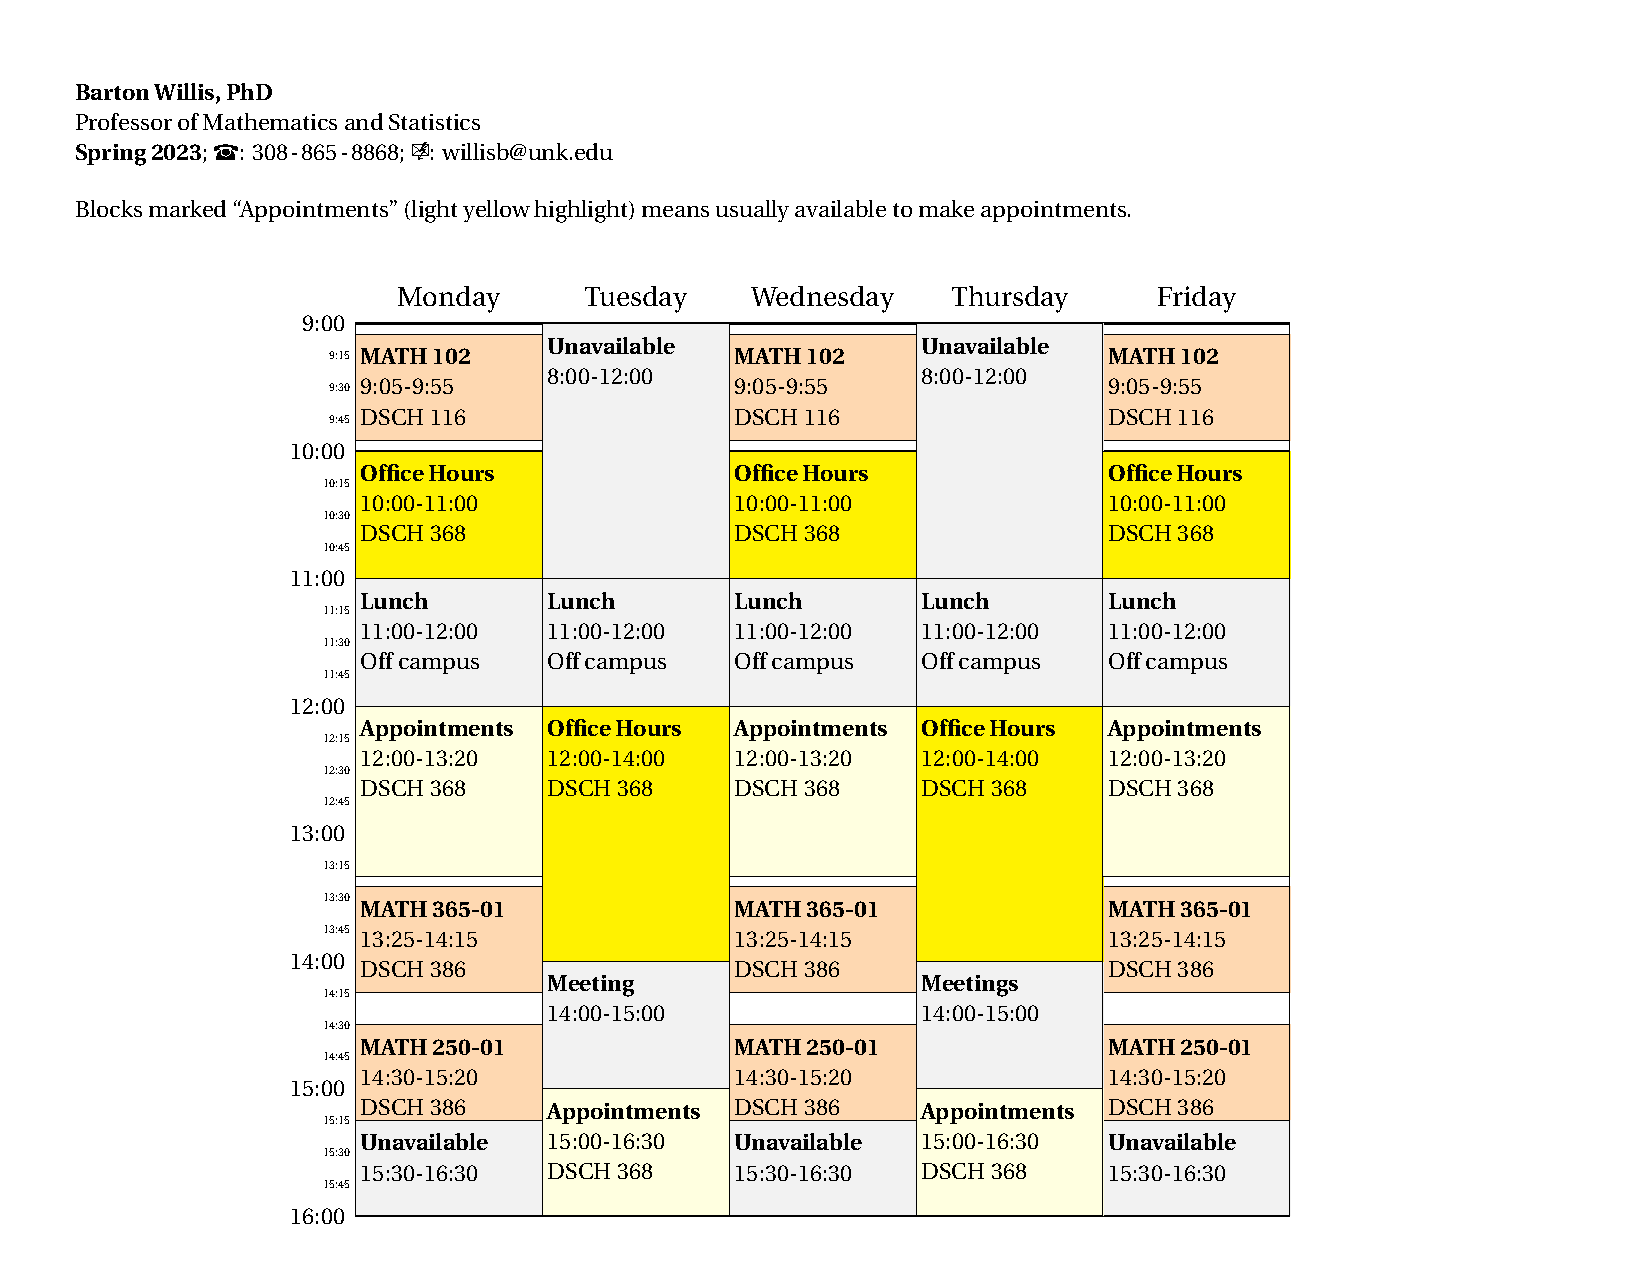
\includepdf[pages={1-},angle=90]{door-schedule.pdf}
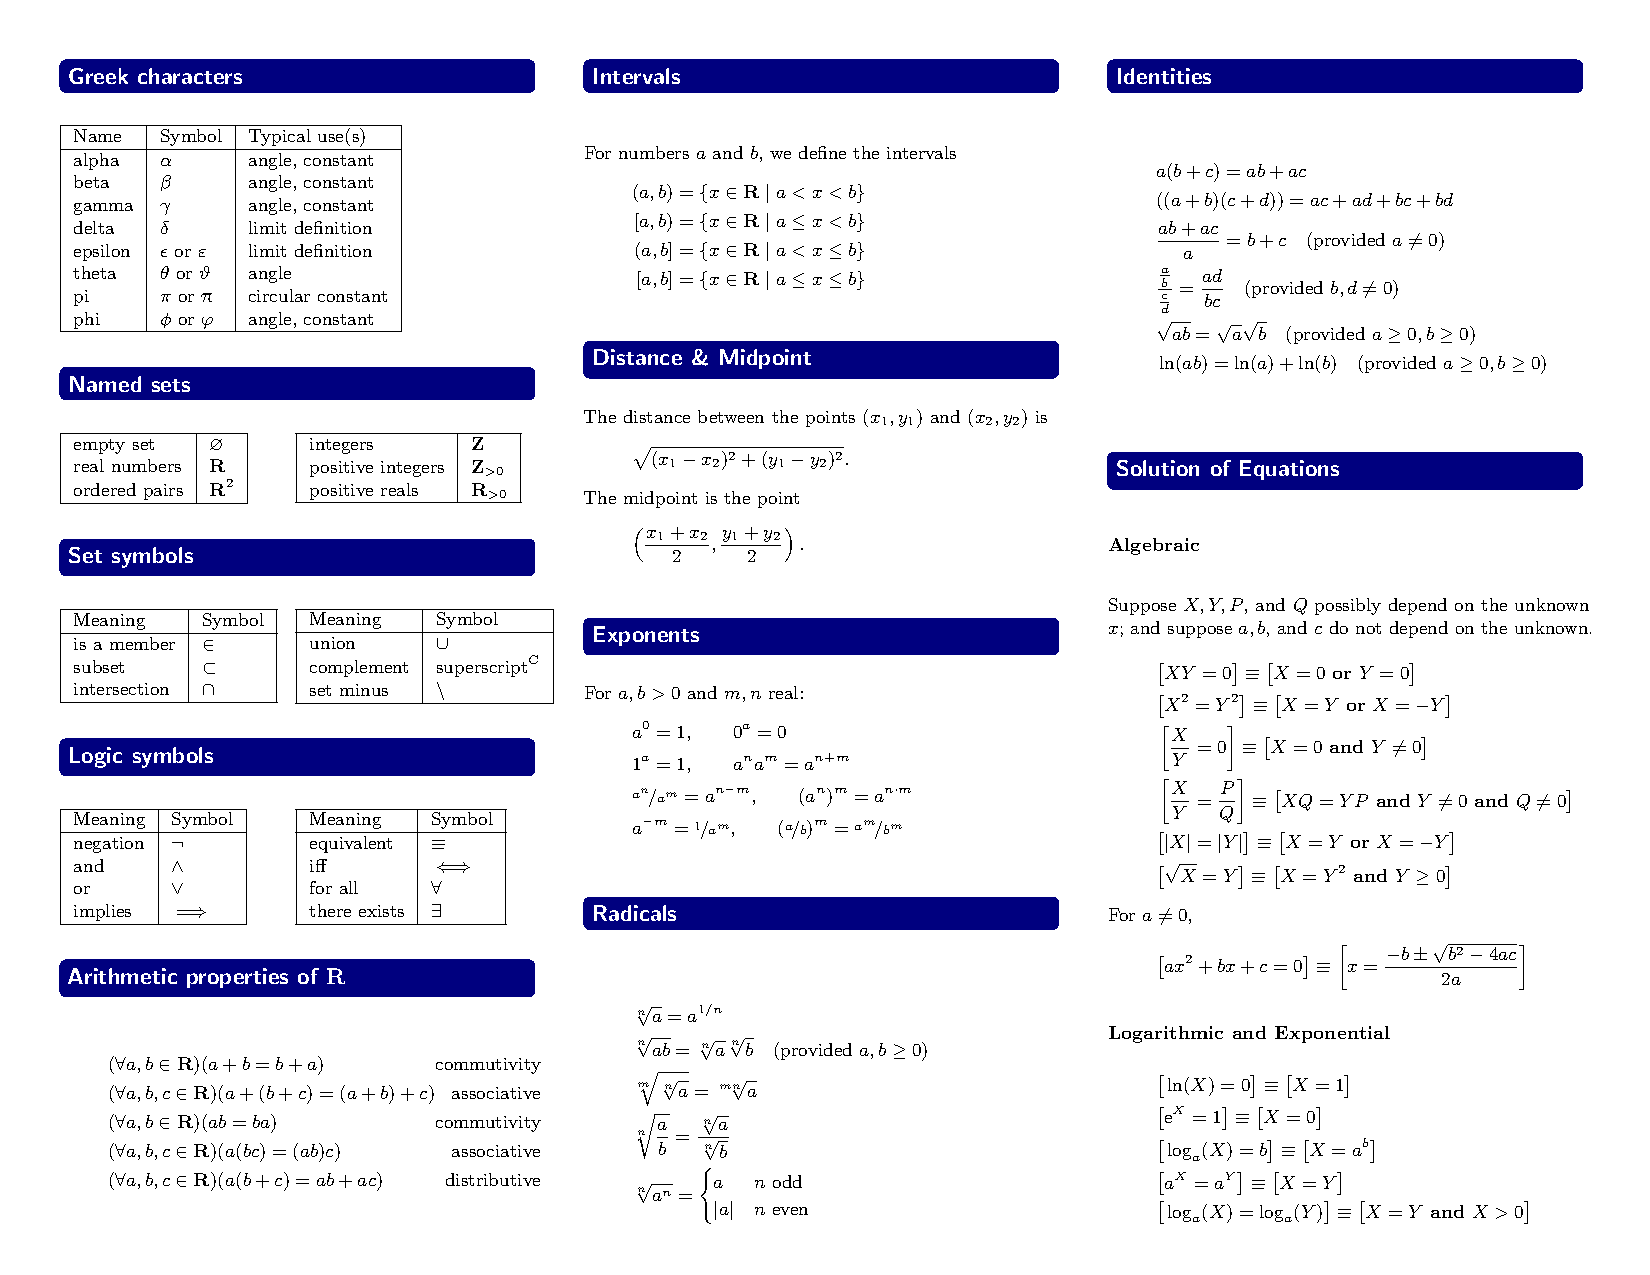
\includepdf[pages={1-},angle=90]{college-algebra-quick-reference.pdf}

\end{document}

